\documentclass[11pt]{article}
\usepackage[T1]{fontenc}
\usepackage[utf8]{inputenc}
\usepackage{lmodern,amsmath,amssymb,graphicx,geometry,microtype,setspace,booktabs,caption}
\usepackage[hidelinks]{hyperref}
\geometry{letterpaper,margin=1in}
\setlength{\parindent}{0pt}
\setlength{\parskip}{0.55em}
\setlength{\emergencystretch}{2em}
\captionsetup{labelfont=bf,font=small}
\renewcommand{\refname}{References}

\pagestyle{empty}
\renewcommand{\thefigure}{S\arabic{figure}}
\setcounter{figure}{3}

\begin{document}
\begin{figure}[!ht]\centering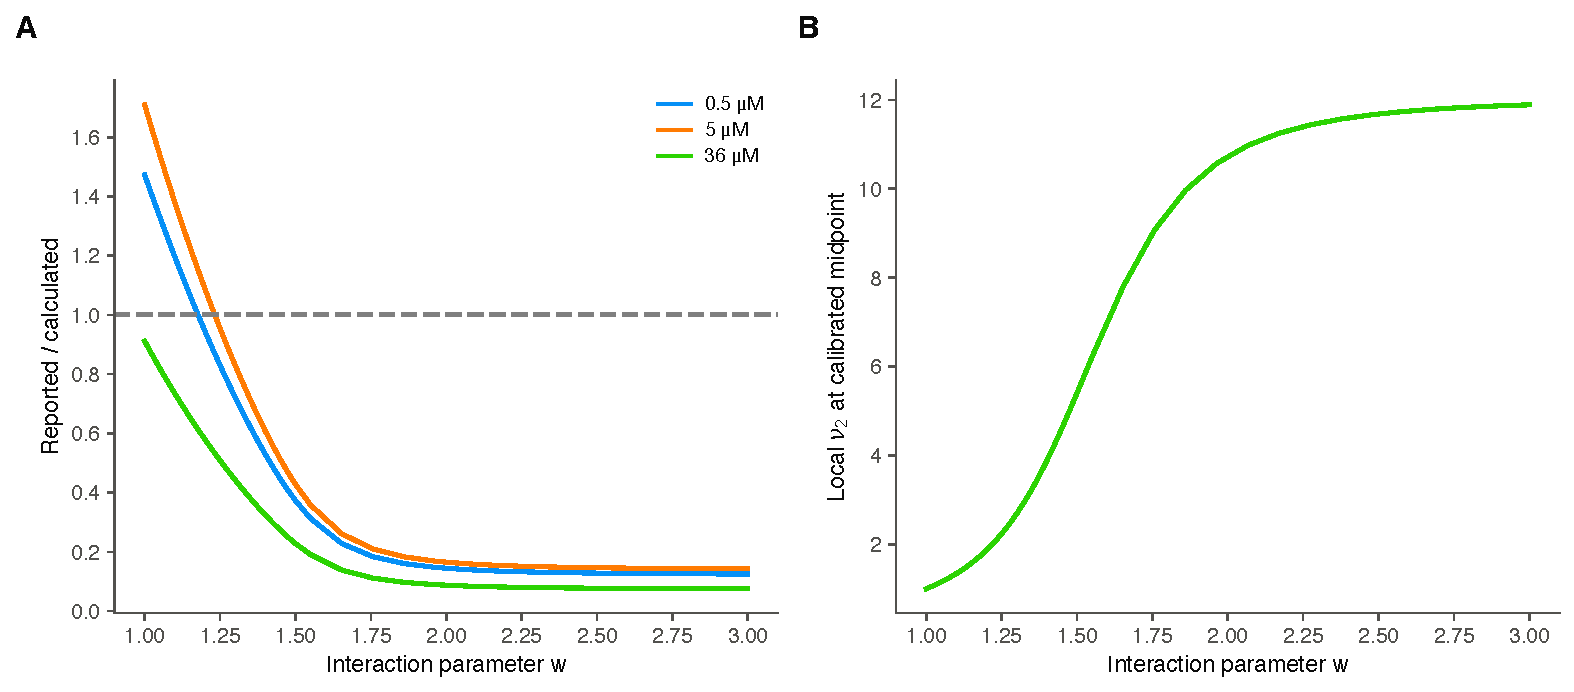
\includegraphics[width=\textwidth,height=0.65\textheight,keepaspectratio]{figure_inputs/FigS4_downstream.pdf}\begin{singlespace}\caption{Downstream ladder interactions and condition-specific local factors. (A) Reported-to-calculated response-range ratios versus the interaction parameter w in Eq. (S28). Each condition has its own calibrated midpoint. (B) The corresponding local ladder factors at those midpoints. These factors need not coincide and are not replaced by their average. Increasing w does not automatically fit every condition jointly. Curves are illustrative calculations, not fitted microscopic interaction strengths.}\end{singlespace}\end{figure}
\end{document}
